The event panel presents the user with a drop-down menu with a list of available event applications. Event applications are applications that, given the building and user supplied data to the specific
applications input panel, will generate a list of events for the building. There are a number of options available in the pull-down menu.


\subsection{Multiple Existing}

This is provided for the user to specify multiple existing SimCenter
Event files.  If more than one event is specified it is done to provide
the UQ engine with a discrete set of events to choose from.  It is not
done with the intention of specifying that one event follows another.
The panel presented initially to the user is as shown
in \autoref{fig:figure4}.

\begin{figure}[!htbp]
  \centering {
    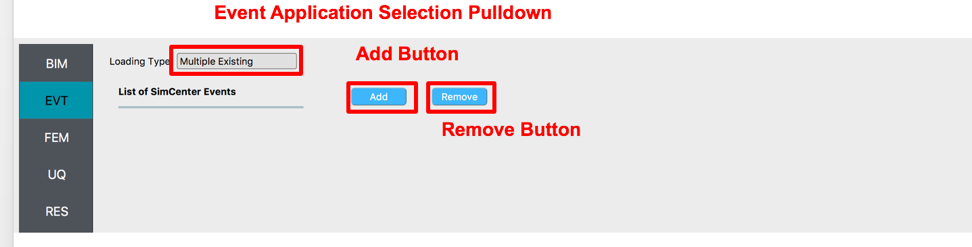
\includegraphics[width=0.8\textwidth]
    {figs/Figure4.png} }
  \caption{EVT}
  \label{fig:figure4}
\end{figure}

To add a new event, the user presses the Add button.  This adds an event to the panel.  Pressing the button multiple times will keep adding events to the panel.  \autoref{fig:figure5} shows the state after the button has been pressed twice, and data entered for the ElCentro and Rinaldi Events.

\begin{figure}[!htbp]
  \centering {
    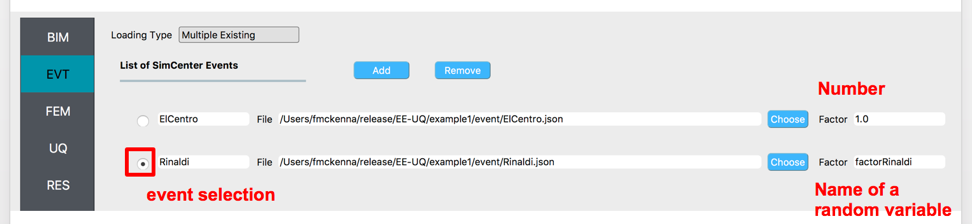
\includegraphics[width=0.8\textwidth]
    {figs/Figure5.png} }
  \caption{Adding new event}
  \label{fig:figure5}
\end{figure}


The user can enter the full path manually to the file or use the choose button,  which brings up your typical file search screen.  By default, a scaling factor of 1.0 is assigned to the event. 
The user can change this to another real value (AT PRESENT DO NOT USE INTEGER) or the user 
has the option of defining this to be a random variable by entering a name as shown for the second event. 

Note that this variable name must not start with a number, or contain any spaces or special characters, i.e. no -, +,..

The Remove button is pressed to remove events. To remove an event the user must first select
which events they wish to remove, done by clicking in the small circle at the start of the event. Once the events to remove  have been selected, the user removes all these selected evens by pressing the remove button.

If the user has multiple events to load, all the event files may first be placed by the user into a seperate folder. If the user presses the  Load Directory, the user will be able to choose a directory and the application will load all the event file (any file with a .json suffix) into the widget by choosing the directory. Initially each event will be given a load factor of 1.0.  Should the user include in that directory a file named Records.txt the application will open that file and load the events and assigned load factors from that file. Each line in Recors.txt is considered ro represent a record, and contains 2 comma seperated values: the first value being the event file and the second value the event factor. An example Records.txt is as shown below:

\begin{verbatim}
ElCentro.json,1.5
Rinaldi.json,2.0
\end{verbatim}

Random Variables: The user can, as mentioned, enter a string in the factor field to specify that the factor is to be considered a random variable. Subsequently in the UQ panel the user must provide information on the random variables distribution. Also, if multiple events are specified, the event itself will be treated as a random variable, with each event being part of the discrete set of possible events.

\subsection{Multiple PEER Event}
This is provided for the user to specify multiple existing PEER 
(\href{http://peer.berkeley.edu}{http://peer.berkeley.edu}) ground motion files. 
For PEER events the user is required to specify the individual components for the EVENTS. 
The Add/Remove buttons at the top are to create and remove an event, as per 2.2.1. 
For the PEER events the user specifies components acting in the individual degree-of-freedom directions. 
The + and – add and remove components with the remove removing all components selected. 
Each component in a PEER event can have their own scale factor, again a number or a random variable.

\begin{figure}[!htbp]
  \centering {
    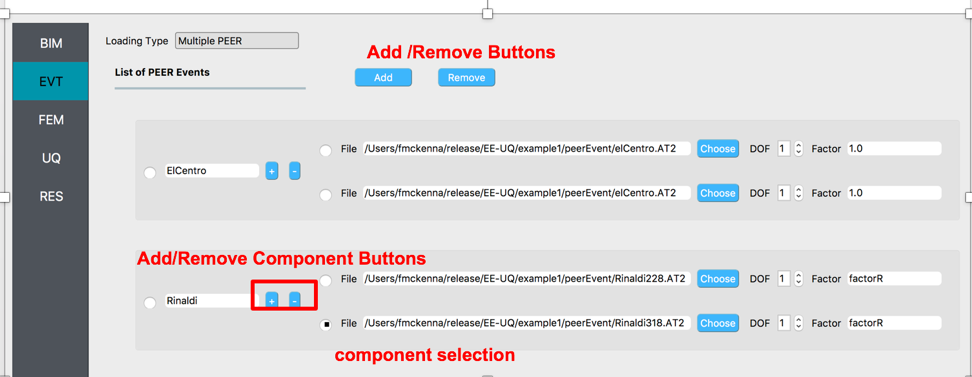
\includegraphics[width=0.8\textwidth]
    {figs/Figure6.png} }
  \caption{PEER event}
  \label{fig:figure6}
\end{figure}

If the user has multiple events to load the user can again place att the PEER .AT2 files into a separate folder and select the Load Directory option. This will allow the user to select a directory. Once selected all .AT2 files in that directory will be loaded into the application. Similar to loading multiple SimCenter events, should the user provide a file Records.txt in that directory, the application will load all files in the list and set the appropriate load factor. An example Results.txt file for multiple Peer events is as shown below:

\begin{verbatim}
elCentro.AT2,1.5
Rinaldi228.AT2,2.0
Rinaldi318.AT2,2.0
\end{verbatim}

Random Variables: The user can, as mentioned, enter a string in the factor field to specify that the factor is to be considered a random variable. Subsequently in the UQ panel the user must provide information on the random variables distribution. Also, if multiple events are specified, the event itself will be treated as a random variable, with each event being part of the discrete set of possible events.

\subsection{Hazard Based Event}
The panel for this event application is as shown
in \autoref{fig:figure7}.  This application implements a
scenario-based (deterministic) seismic event.  In this panel the user
specifies an earthquake rupture (location, geometry and magnitude), a
ground motion prediction equation, a record selection database and the
intensity measure used for record selection.  In the backend, this
application relies on three other applications to perform seismic
hazard analysis, intensity measures simulation (to create a simulated
target spectrum), and ground motion record selection/scaling.  Users
interested in learning about those applications are referred to the
documentation of the
(\href{https://github.com/NHERI-SimCenter/GroundMotionUtilities/blob/master/Readme.md}{SimCenter
ground motion utilities}).
\begin{figure}[!htbp]
  \centering {
    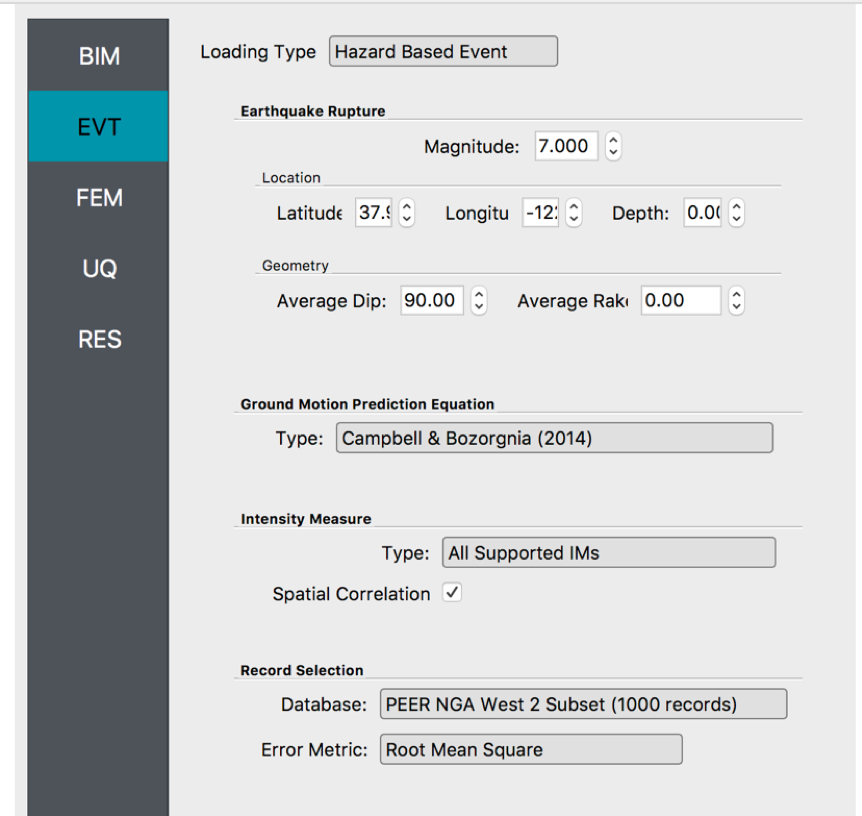
\includegraphics[width=0.8\textwidth]
    {figs/Figure7.png} }
  \caption{Hazard based event}
  \label{fig:figure7}
\end{figure}

\subsection{Stochastic Ground Motion Model}
This option allows users to generate synthetic ground motions for a
target seismic event. In order to do so, the stochastic ground motion
model is selected from the drop-down menu, as shown
in \Cref{fig:stochastic_loading}. Depending on the model selected, the
user will be asked to enter values for a number of parameters that are
used to generate a seismic event. In the current release, users can
select between the model derived by Vlachos et
al. (2018) \cite{vlachos2018predictive} and the model developed by
Dabaghi \& Der Kiureghian (2014, 2017, 2018)
[\cite{dabaghi2014stochastic}, \cite{dabaghi2017stochastic}, \cite{dabaghi2018simulation}]. Additionally,
users can provide a seed for the stochastic motion generation if they
desire the same suite of synthetic motions to be generated on multiple
occasions.  If the seed is not specified, a different realization of
the time history will be generated for each run. The backend
application that generates the stochastic ground motions relies
on \texttt{smelt}, a modular and extensible C++ library for generating
stochastic time histories. Users interested in learning more about the
implementation and design of
\texttt{smelt} are referred to its
\href{https://github.com/NHERI-SimCenter/smelt}{GitHub repository}.

All input parameters can be specified as random variables by entering
a string in the parameter field. Please note that information for the
inputs that are identified as random variables needs to be provided in
the \texttt{UQ} tab.

\begin{figure}[!htbp]
  \centering {
    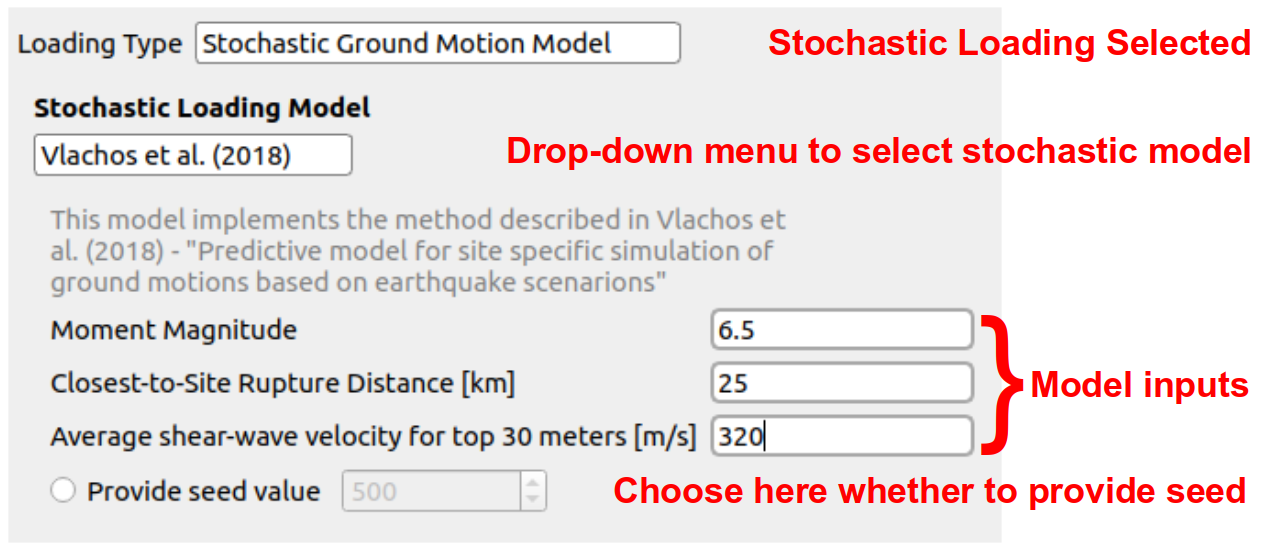
\includegraphics[width=0.8\textwidth]
    {usage/figures/stochastic_loading.png} }
  \caption{Stochastic Ground Motion Event}
  \label{fig:stochastic_loading}
\end{figure}




\subsubsection{s$^3$hark}
The panel for this event application is as shown in \autoref{fig:s3hark0}. 
This application does effective free-field site response analysis of a soil column.
In this panel the user specifies a ground motion at the bottom of the column. 
With soil layer properly defined, the motion at the ground surface will be given at the end of the analysis.
\begin{figure}[!htbp]
  \centering {
    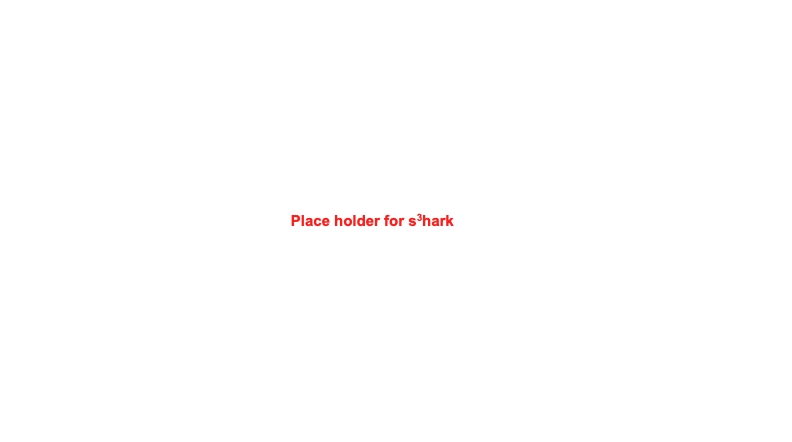
\includegraphics[width=0.8\textwidth]
    {figs/s3hark0.png} }
  \caption{s$^3$hark}
  \label{fig:s3hark0}
\end{figure}

The UI of s$^3$hark is shown in \autoref{fig:s3hark1}.
There are two graphics shown in the left of the panel. The first one is the soil column graphic, 
which shows a visualization of the soil column.
The second one is the mesh and profile graphic, 
which shows the finite element mesh and profile plots.
On the right of the panel are operation area, soil design table, configure tab, layer property tab and response tab. 


\begin{figure}[!htbp]
  \centering {
    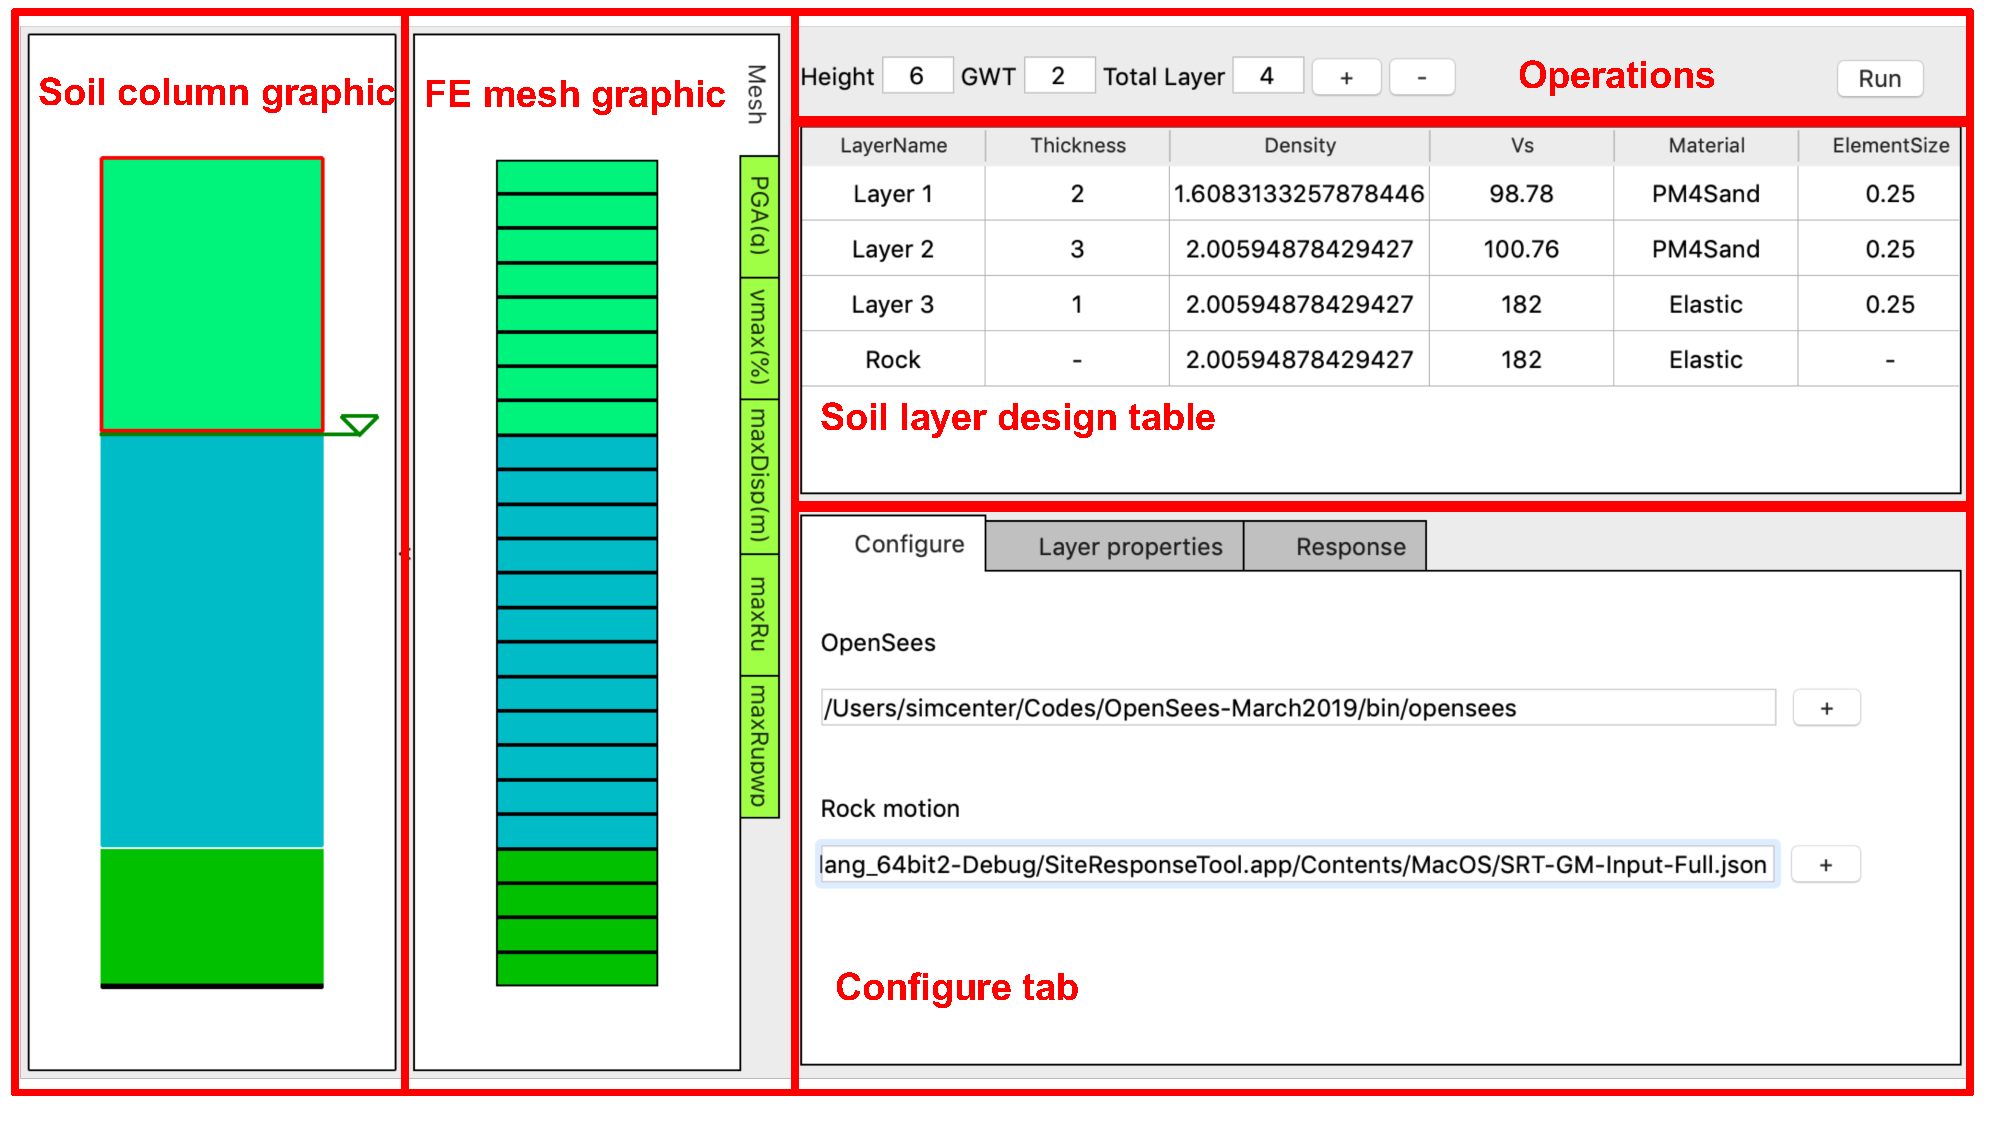
\includegraphics[width=0.8\textwidth]
    {figs/s3hark1.pdf} }
  \caption{s$^3$hark - Panels}
  \label{fig:s3hark1}
\end{figure}

In the operation area as shown in \autoref{fig:s3hark2}, click the plus button to add a layer and the minors button to delete a selected layer. 
Change the ground water table in the GWT input field. 
In the configure tab, path of OpenSees executable and rock motion file need to be specified.
A click on the run button will start the finite element analysis.


\begin{figure}[!htbp]
  \centering {
    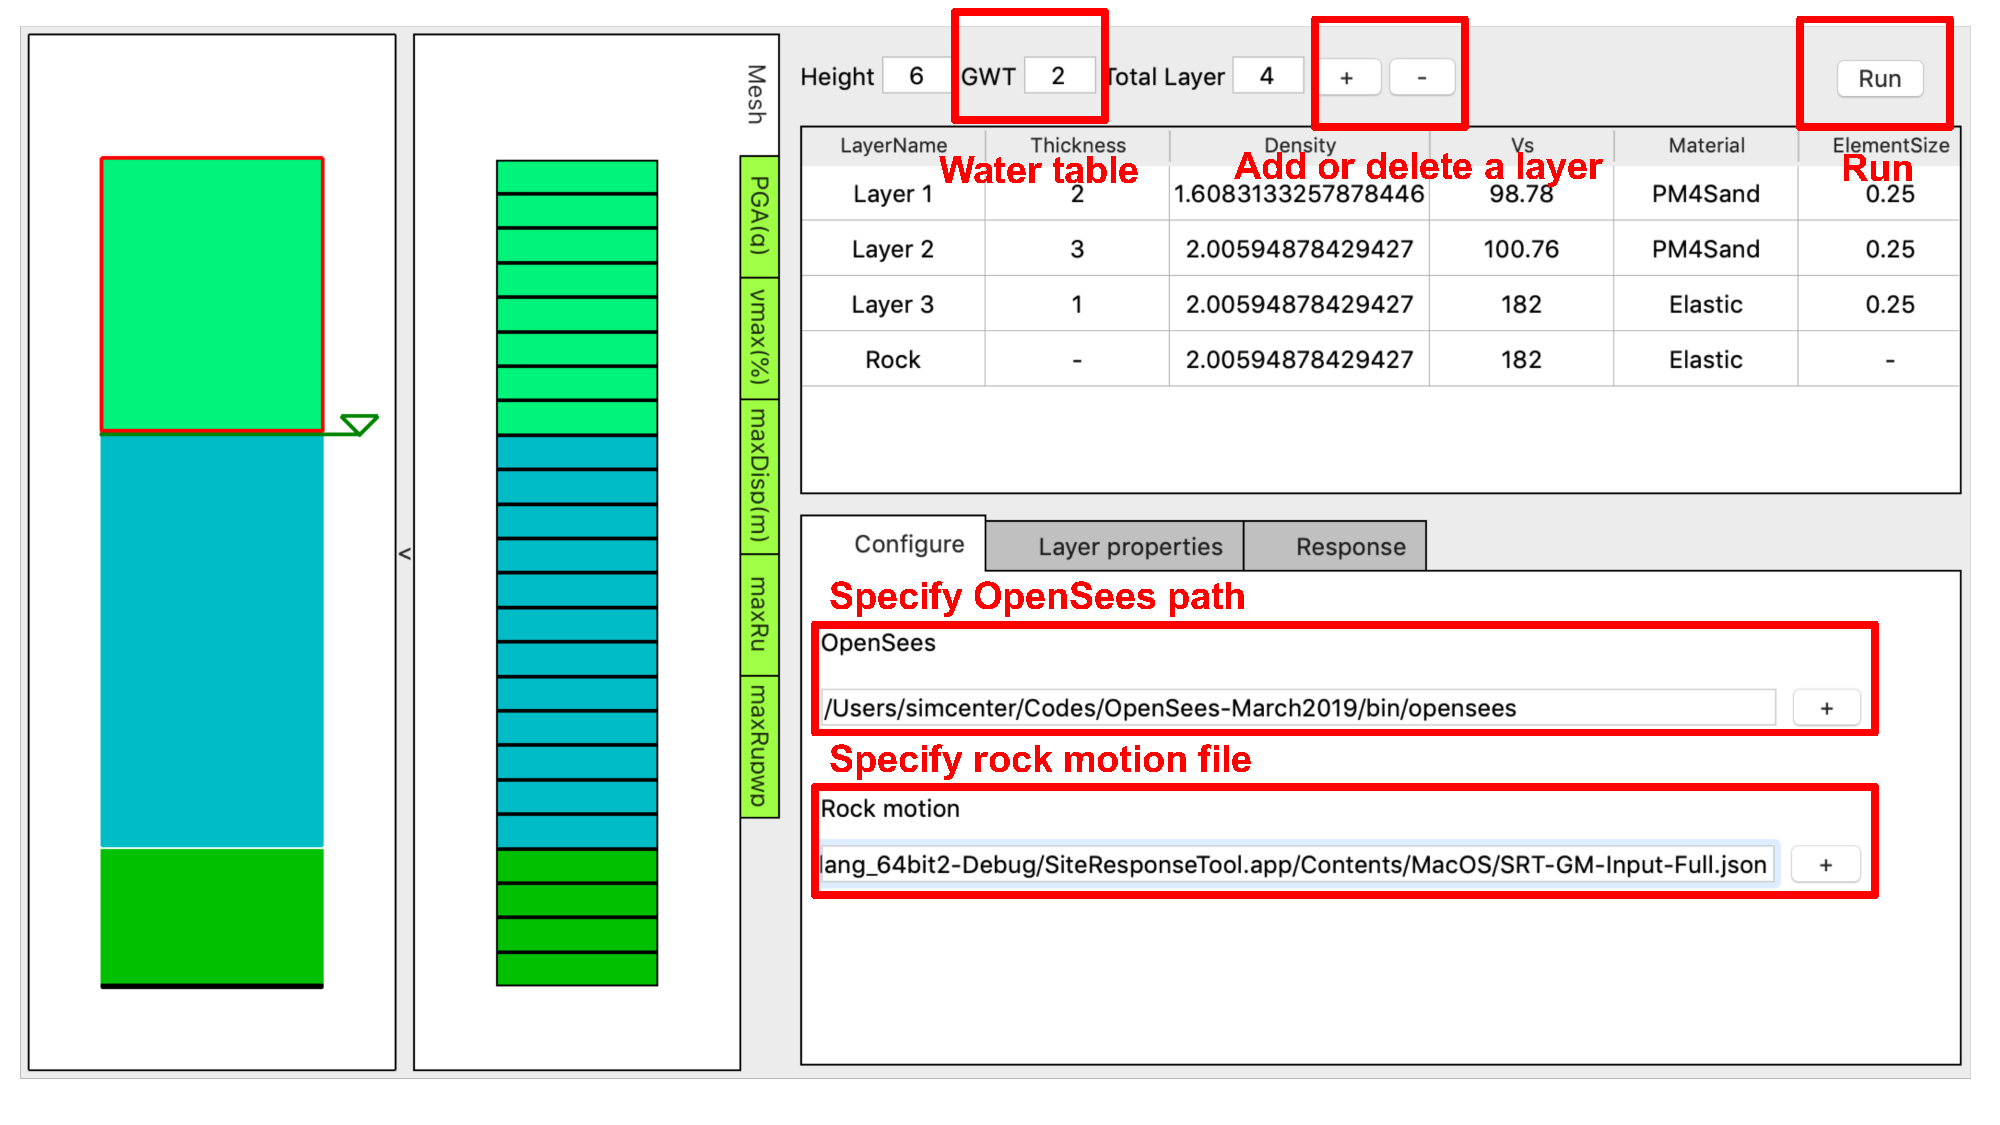
\includegraphics[width=0.8\textwidth]
    {figs/s3hark2.pdf} }
  \caption{s$^3$hark - Configurations and Operations }
  \label{fig:s3hark2}
\end{figure}

Either click on the soil column or the table to select a layer \autoref{fig:s3hark3}. 
When a layer is selected, it will be highlighted in both the soil column graphic and the table. 
Selection of a soil layer will invoke the Layer properties tab, where the user can specify the material properties of this layer.
Double click on a cell of the table will allow the user to change the corresponding value.

\begin{figure}[!htbp]
  \centering {
    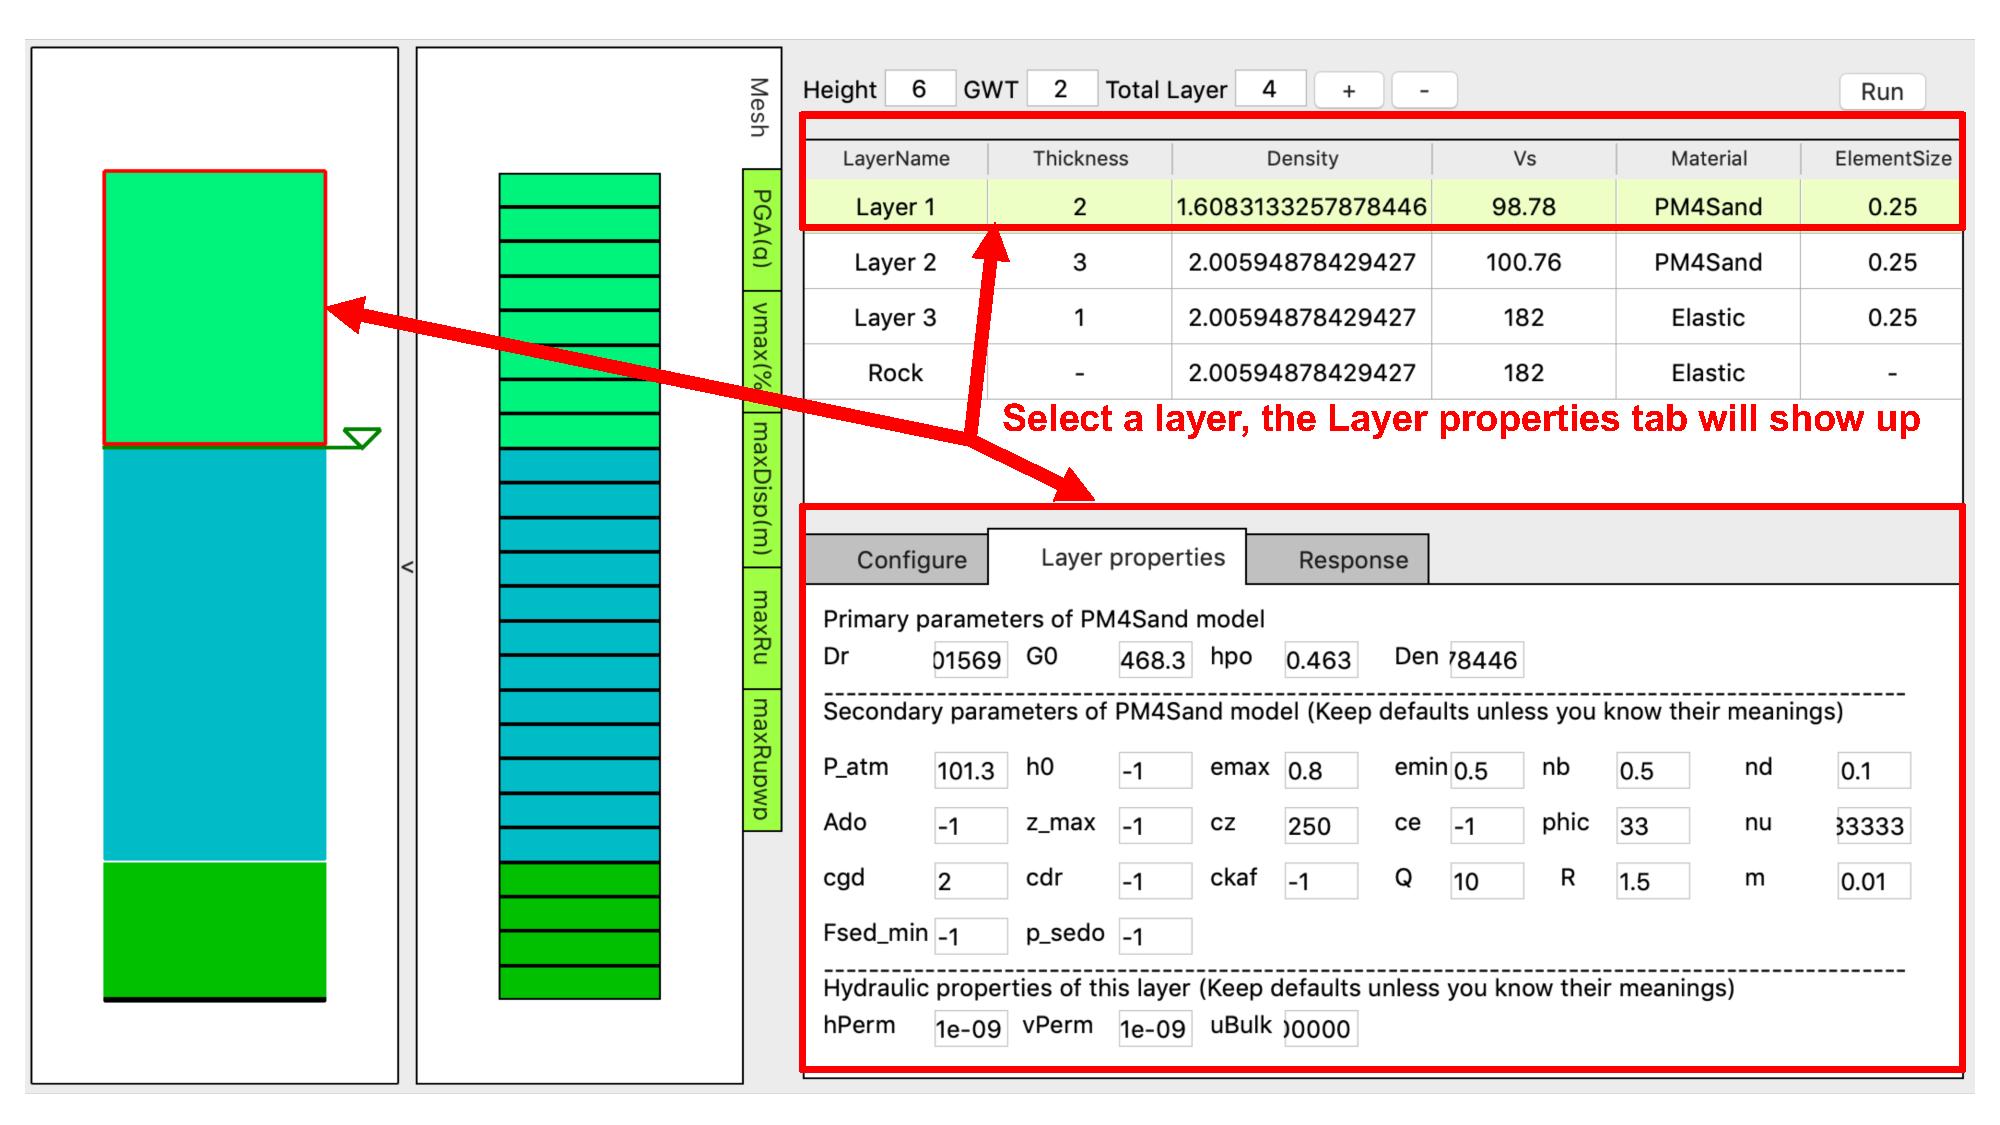
\includegraphics[width=0.8\textwidth]
    {figs/s3hark3.pdf} }
  \caption{s$^3$hark - Layer modification }
  \label{fig:s3hark3}
\end{figure}


Upon the finish of the finite element analysis, the ground motion at the soil surface (\autoref{fig:s3hark4}) will be stored in EE-UQ's input file.
This computed motion will be later applied to the bottom of the building.

\begin{figure}[!htbp]
  \centering {
    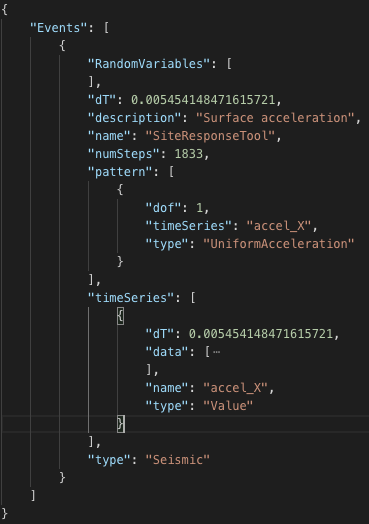
\includegraphics[width=0.4\textwidth]
    {figs/s3hark4.png} }
  \caption{s$^3$hark - Surface motion }
  \label{fig:s3hark4}
\end{figure}












\subsection{User Application}
The final selection option is a user specific application. 
The user specifies the application name and the input file containing the specific input information 
needed by the application when it is running in the backend. 
As will be discussed, the user is also required when they use an additional application not provided, 
to edit the tools registry file. Here they must include a new event application with this same name 
and the location where that application can be found relative to the tools application directory. 
If running on DesignSafe, that application must of course be built and available on the Stampeded2 supercomputer. 
NOTE that given how DesignSafe runs the applications through Agave, this applications file permissions must be 
world readable and executable (as when user running their application through DesignSafe and Agave, they are not running as themselves!)

\begin{figure}[!htbp]
  \centering {
    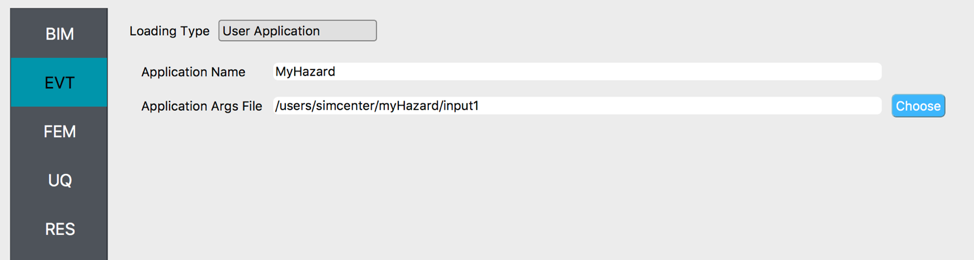
\includegraphics[width=0.8\textwidth]
    {figs/Figure8.png} }
  \caption{User defined event}
  \label{fig:figure8}
\end{figure}


